\section{\large PLANTEAMIENTO DEL PROBLEMA}
	
	\subsection{Enunciado del problema}

La Organización para la Cooperación y el Desarrollo Económicos (2018), afirma que “la desigualdad económica es el distinto reparto de los ingresos, los activos o el bienestar entre el conjunto de habitantes”.

Latino américa es la región más desigual de la región en términos socio económicos; según Lustig (2011), “la región latinoamericana es 19\% más desigual que el África subsahariana, 37 más desigual que el este asiático y 65\% más desigual que los países desarrollados”.  En efecto América Latina es, hoy, la región sin guerras más desigual del planeta: más que India, más que algunos países de África Subsahariana.

La desigualdad socio económica impide luchar contra la pobreza, ampara a los grupos vulnerables de vivir en la pobreza sin acceso a un trabajo decente, servicios básicos, exposición a una nutrición malsana o falta de vivienda digna. Se excluye el estatus social y los individuos y familias continúan existiendo.

En este sentido es evidente la importancia de entender la pobreza. \cite{Ravallion1991}, afirman que la pobreza alude a niveles de vida.  " Esto es: ¿cuántas personas no pueden satisfacer ciertas necesidades predeterminadas de consumo y acceso amplio a bienes públicos (servicios de salud, educación, vivienda)?" 

Según el Instituto Nacional de Estadística e Informática (2000) “La pobreza es una condición en la cual una o más personas tienen un nivel de bienestar inferior al mínimo socialmente aceptado.” 

Las estadísticas indican que desde el año 2000 se ha conseguido reducir la tasa de incidencia de la pobreza en el Perú.
El siguiente cuadro del Banco Mundial se presenta la tasa de incidencia de la pobreza, en relación a la base de la línea de pobreza nacional (\% de la población) para el periodo 2004 – 2019

\begin{figure}[H]
    \caption{Tasa de incidencia de la pobreza, sobre la base de la línea de pobreza nacional (\% de la población) – Perú.}
    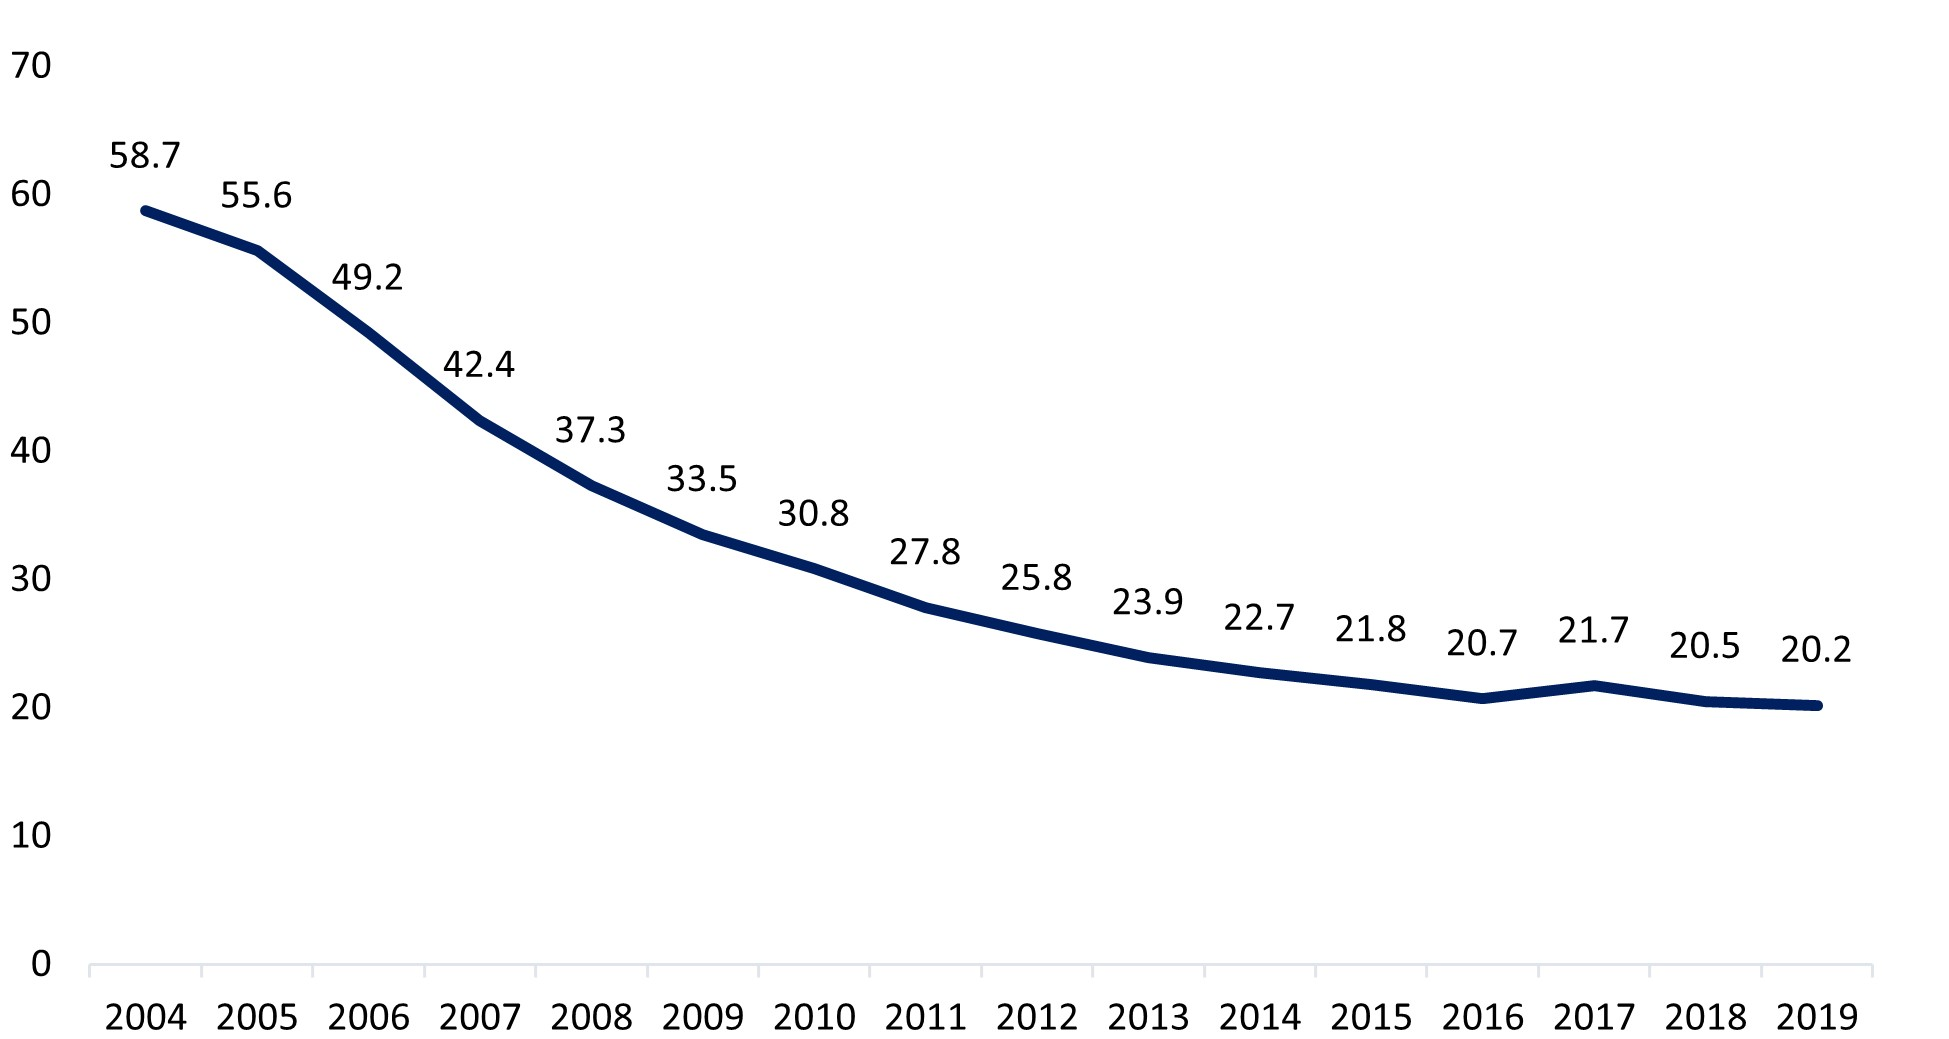
\includegraphics[scale=0.8]{Images/Ch_1_Planteamiento_problema/Imagen1.jpg}
    \label{fig:Figure1}  
    
     \begin{tablenotes}[para,flushleft]
     {\small
         \textit{Note.} Elaboración propia, Banco mundial.
     }
     \end{tablenotes}
\end{figure}

Donde precisa que la tasa de incidencia de la pobreza entre 2004 y 2019 se redujo en 38.5\%. señala también que el principal periodo de reducción fue entre 2004 y 2011. 

Los años 2002 a 2016 la tasa de pobreza bajo de 54,30\% a 20,7\% y la extrema pobreza de 24.2\% a 3.8\%, ya que, en los gobiernos de Alejandro Toledo, Alan García y Ollanta Humana la tasa de pobreza se redujo en 5,2\%, 21,4\%, 7,03\% y la extrema pobreza en 10,4\%, 7,5\%; 2,54\%, respectivamente, llegando para el año 2018 con 20,50\% de pobreza y 2,8\% de extrema pobreza, con predisposición a seguir descendiendo. 

La tasa de pobreza pasó de 54\% en 1990 a 20,50\% para 2018 y la extrema pobreza de 24.2\% a 2.8\% en el mismo periodo de años, reduciéndose significativamente la pobreza y extrema pobreza en 33,5\% y 21.4\% respectivamente; esto como consecuencia del crecimiento económico sostenido, lo cual implicó un aumento del gasto social, aumento de la inversión pública y una mejora en la calidad y focalización de los programas sociales.

En los periodos 2001 a 2010, la pobreza decreció en 23,5 puntos porcentuales, al pasar de 54,8\% a 31,3\% en el 2010.

\begin{figure}[H]
    \caption{Evolución de la tasa de pobreza, 2001-2010 (\% de la población total).}
    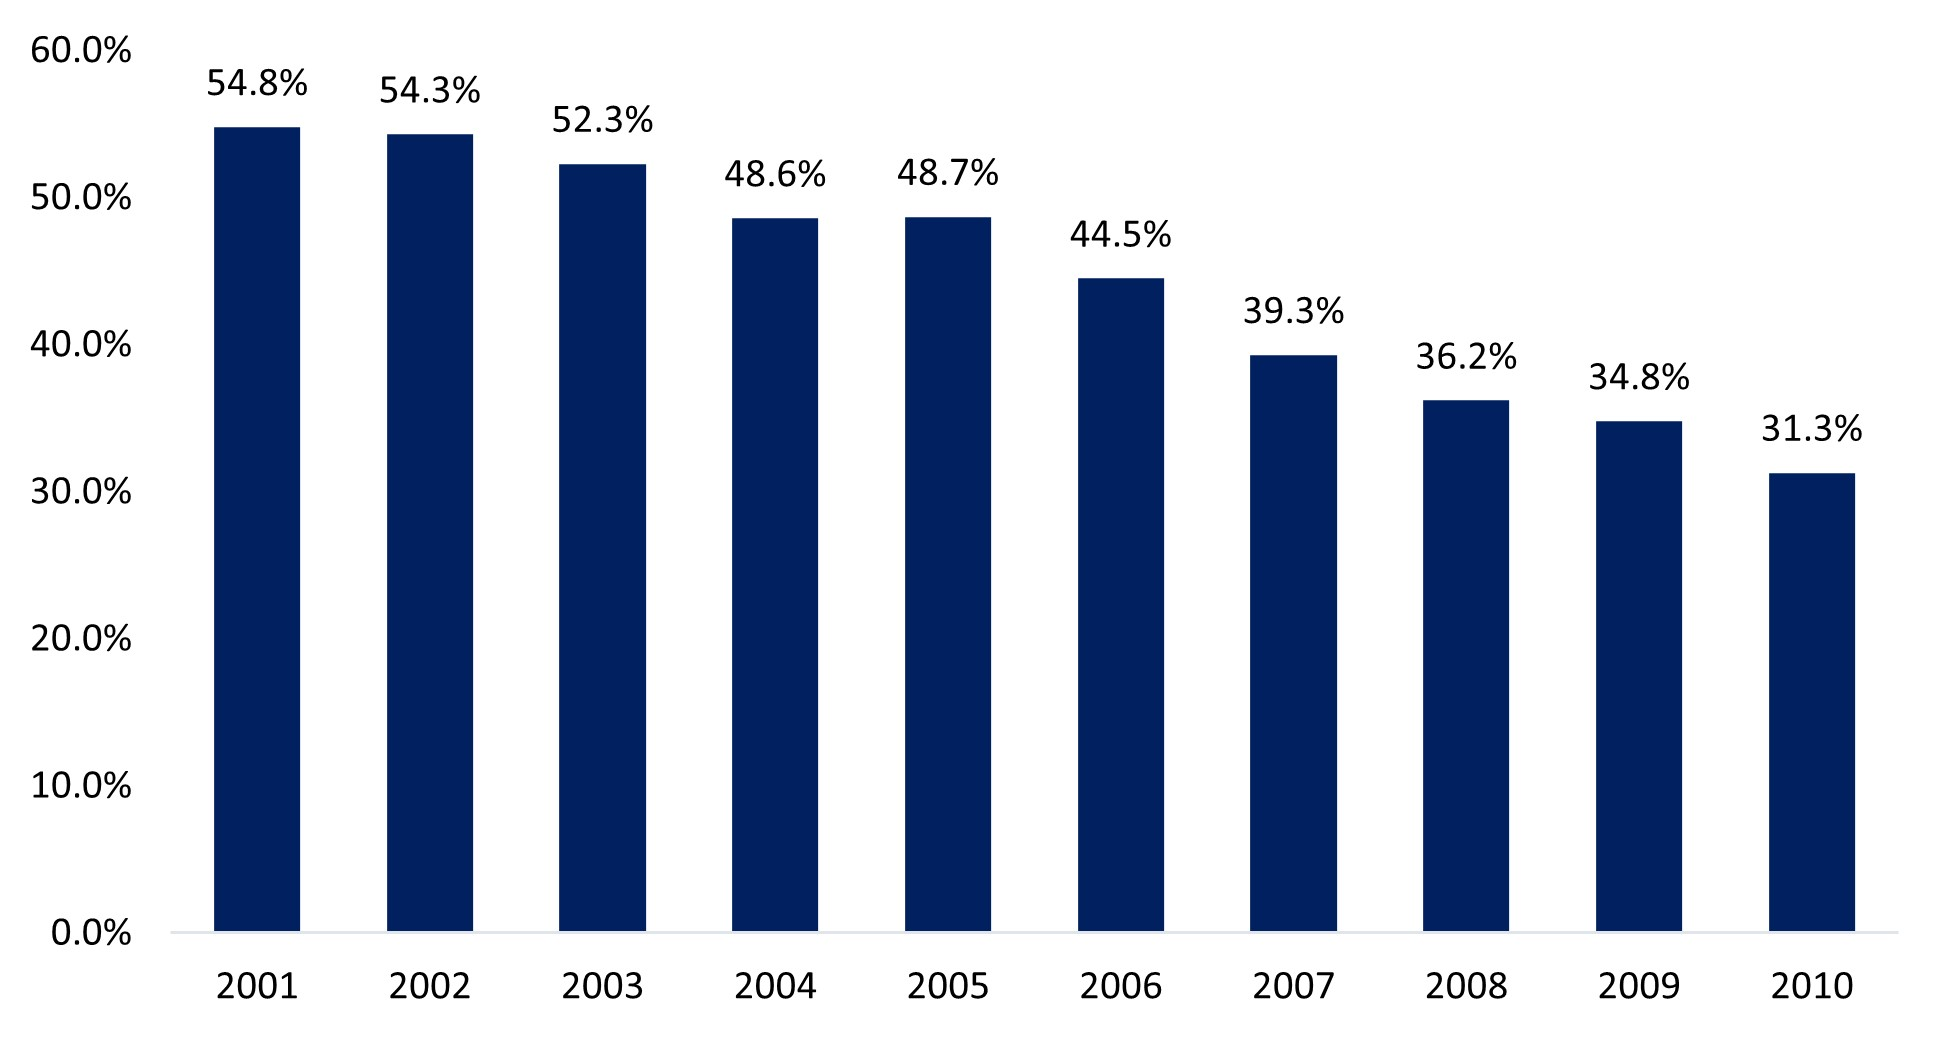
\includegraphics[scale=0.8]{Images/Ch_1_Planteamiento_problema/Imagen2.jpg}
    \label{fig:Figure2}  
    
     \begin{tablenotes}[para,flushleft]
     {\small
         \textit{Note.} Elaboración propia, Banco mundial.
     }
     \end{tablenotes}
\end{figure}

Mientras que en año 2017, 6 millones 906 mil de personas (21,7\%), se encontraban en situación de pobreza, lo que significa que estas personas tenían un nivel de gasto por debajo del costo de la canasta básica de consumo. Comparando este resultado con los niveles del año 2016, se puede observar que la tasa de pobreza ha aumentado en 1,0\%, equivalente a 375.000 pobres, más que en 2016.

\begin{figure}[H]
    \caption{Evolución de la tasa de pobreza, 2001-2010 (\% de la población total).}
    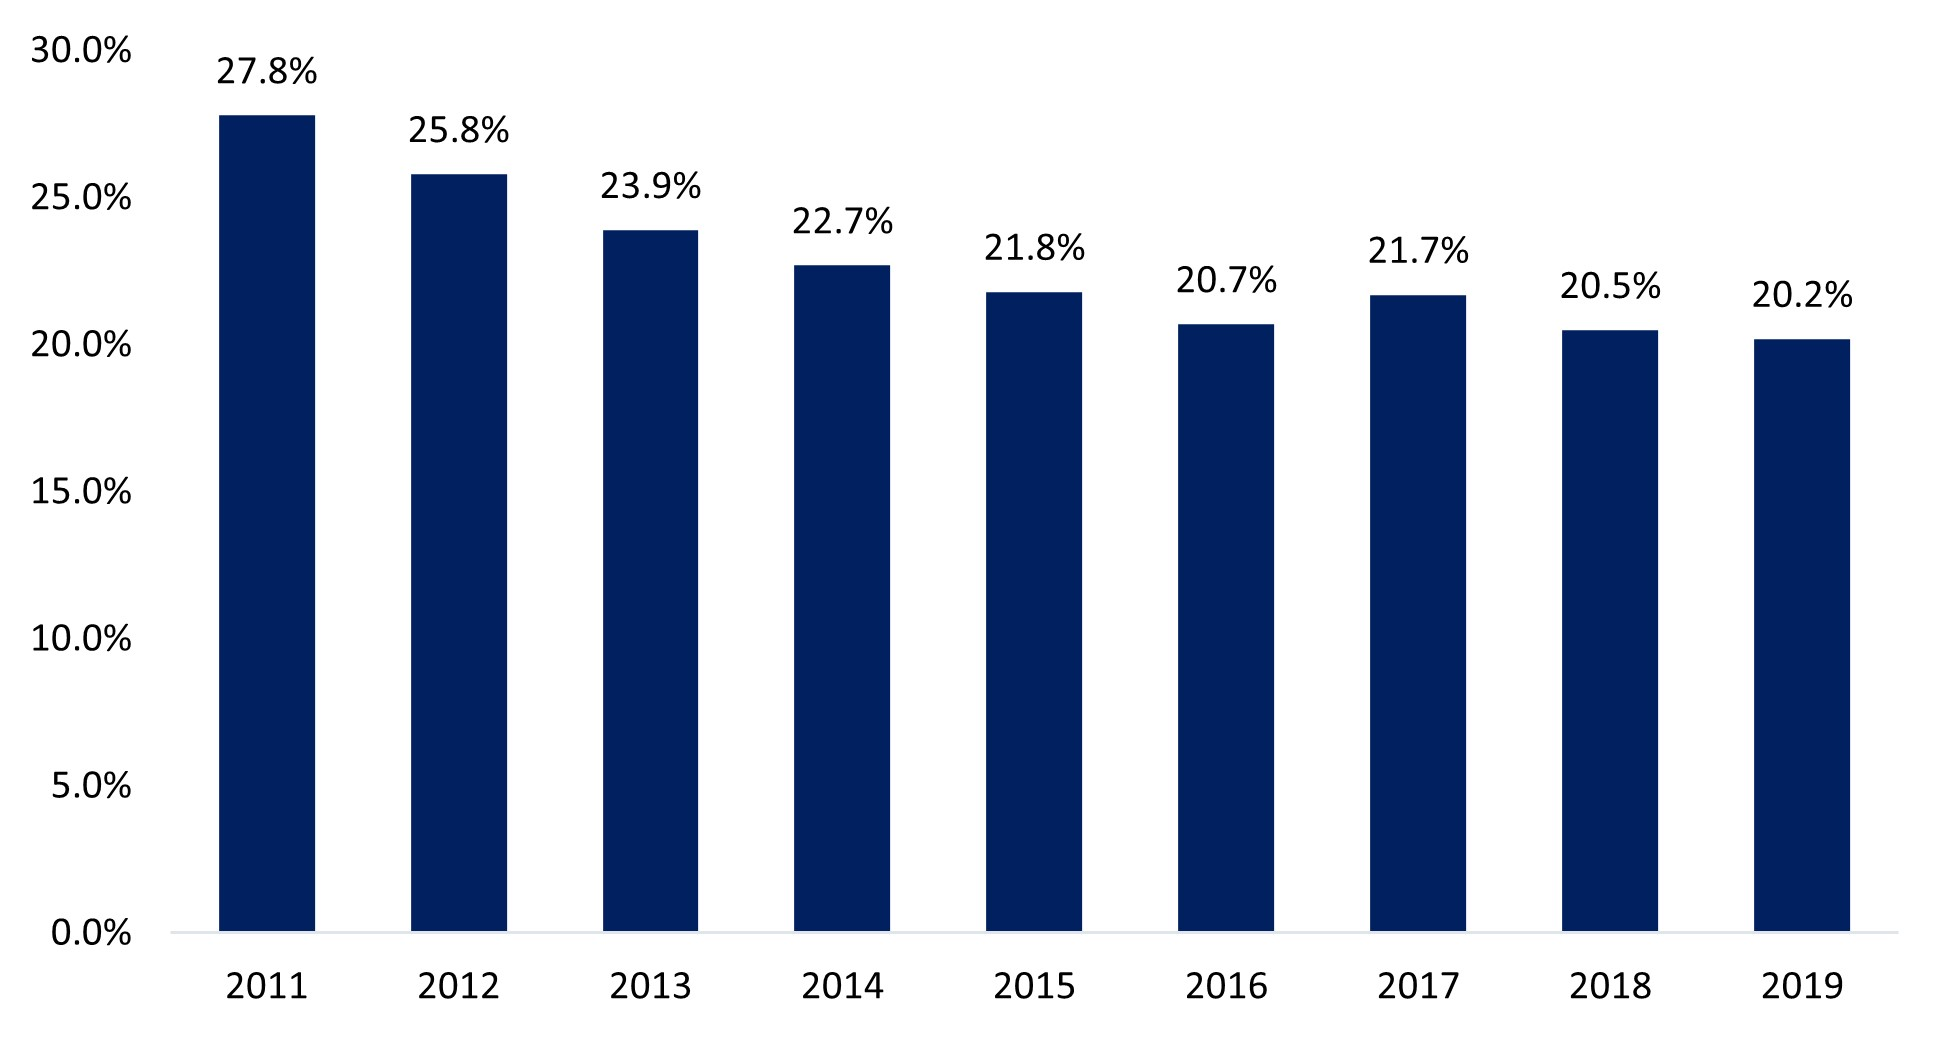
\includegraphics[scale=0.8]{Images/Ch_1_Planteamiento_problema/Imagen3.jpg}
    \label{fig:Figure3}  
    
     \begin{tablenotes}[para,flushleft]
     {\small
         \textit{Note.} Elaboración propia, INEI.
     }
     \end{tablenotes}
\end{figure}

En 2019, el índice de pobreza monetaria afectó al 20,2\% de la población del país, manteniendo casi el mismo nivel que en 2018; Así lo publicó el INEI, de acuerdo con los resultados de la Encuesta Nacional de Hogares (ENAHO) 2019. También señaló que la población en pobreza es considerada la población promedio. el gasto está por debajo del valor de la línea de pobreza (PL), el equivalente monetario de una canasta de productos básicos y alimenticios.

Cuando se habla de pobreza también se hace referencia a la desigualdad social; un grupo social que es excluido ya que no cuenta con el mismo acceso a los recursos que otros grupos con poder si tienen, estas diferencias están marcadas con claridad entre las zonas urbanas y rurales. 

La aplicación errada de políticas públicas ha pronunciado aún más las diferencias, ya que no se ha permitido una integración de la multiculturalidad con la que cuenta el Perú, y muy por el contrario ha ocasionado un marcado distanciamiento entre ellos.

En un contexto de crecimiento económico sostenido, es necesario mejorar la formulación y aplicación de las políticas del país, en objetivos puntuales de desarrollo y asistencia social con el firme objetivo de combatir la pobreza a largo plazo mejorar los estándares de vida de su población en conjunto.


\subsection{Formulación del problema}

\subsubsection{Problema general}

¿Cómo la desigualdad socioeconómica determina el grado de pobreza en el departamento de Ayacucho, periodo 2000-2019?

\subsubsection{Problemas específicos }

\begin{itemize}

\item ¿Cuál es la influencia del empleo en el IDH en el departamento de Ayacucho, periodo 2000-2019?

\item ¿Cuál es la incidencia del índice de Theilen en la determinación de grado de pobreza en el departamento de Ayacucho, periodo 2000-2019?

\item ¿Como el desempleo influye en el índice de Gini en el departamento de Ayacucho, periodo 2000-2019? 

\end{itemize}



